\documentclass[11pt,a4paper]{article}

\usepackage[utf8]{inputenc}
\usepackage[vietnamese,english]{babel}
\usepackage{amsmath,amssymb}
\usepackage{graphicx}
\usepackage{geometry}
\geometry{a4paper, margin=18mm}
\usepackage{booktabs}
\usepackage{float}
\usepackage{hyperref}
\usepackage{xcolor}
\usepackage{fancyhdr}
\usepackage{titlesec}

\hypersetup{
    colorlinks=true,
    linkcolor=blue!70!black,
    urlcolor=blue!70!black
}

\pagestyle{fancy}
\fancyhf{}
\rhead{\small \textit{Hệ thống Nhúng STM32F103 - Smart Room}}
\lhead{\small \textit{Lưu đồ Thuật toán kết hợp Máy trạng thái (Flowchart + HLSM)}}
\rfoot{\thepage}

\titleformat{\section}{\large\bfseries\color{blue!60!black}}{\thesection}{1em}{}

\begin{document}
\selectlanguage{vietnamese}

\begin{center}
    {\LARGE \textbf{BÁO CÁO GIẢI THUẬT \& KIẾN TRÚC ĐIỀU KHIỂN}}\\[1.5mm]
    {\large \textbf{MÔ HÌNH KẾT HỢP FLOWCHART VÀ MÁY TRẠNG THÁI (HLSM)}}\\[1mm]
    {\normalsize \textbf{Hệ thống Giám sát và Điều khiển Phòng thông minh (STM32F103C8T6)}}
    \vspace{2mm}
    \hrule height 1pt
\end{center}

\vspace{1mm}

\section{Sơ đồ Tích hợp Flowchart và HLSM}
Sơ đồ dưới đây biểu diễn trực quan toàn bộ hệ thống: kết hợp giữa **Lưu đồ tiến trình định thời (Cooperative Scheduler)** và **Máy trạng thái mức cao (HLSM)**:

\begin{figure}[H]
    \centering
    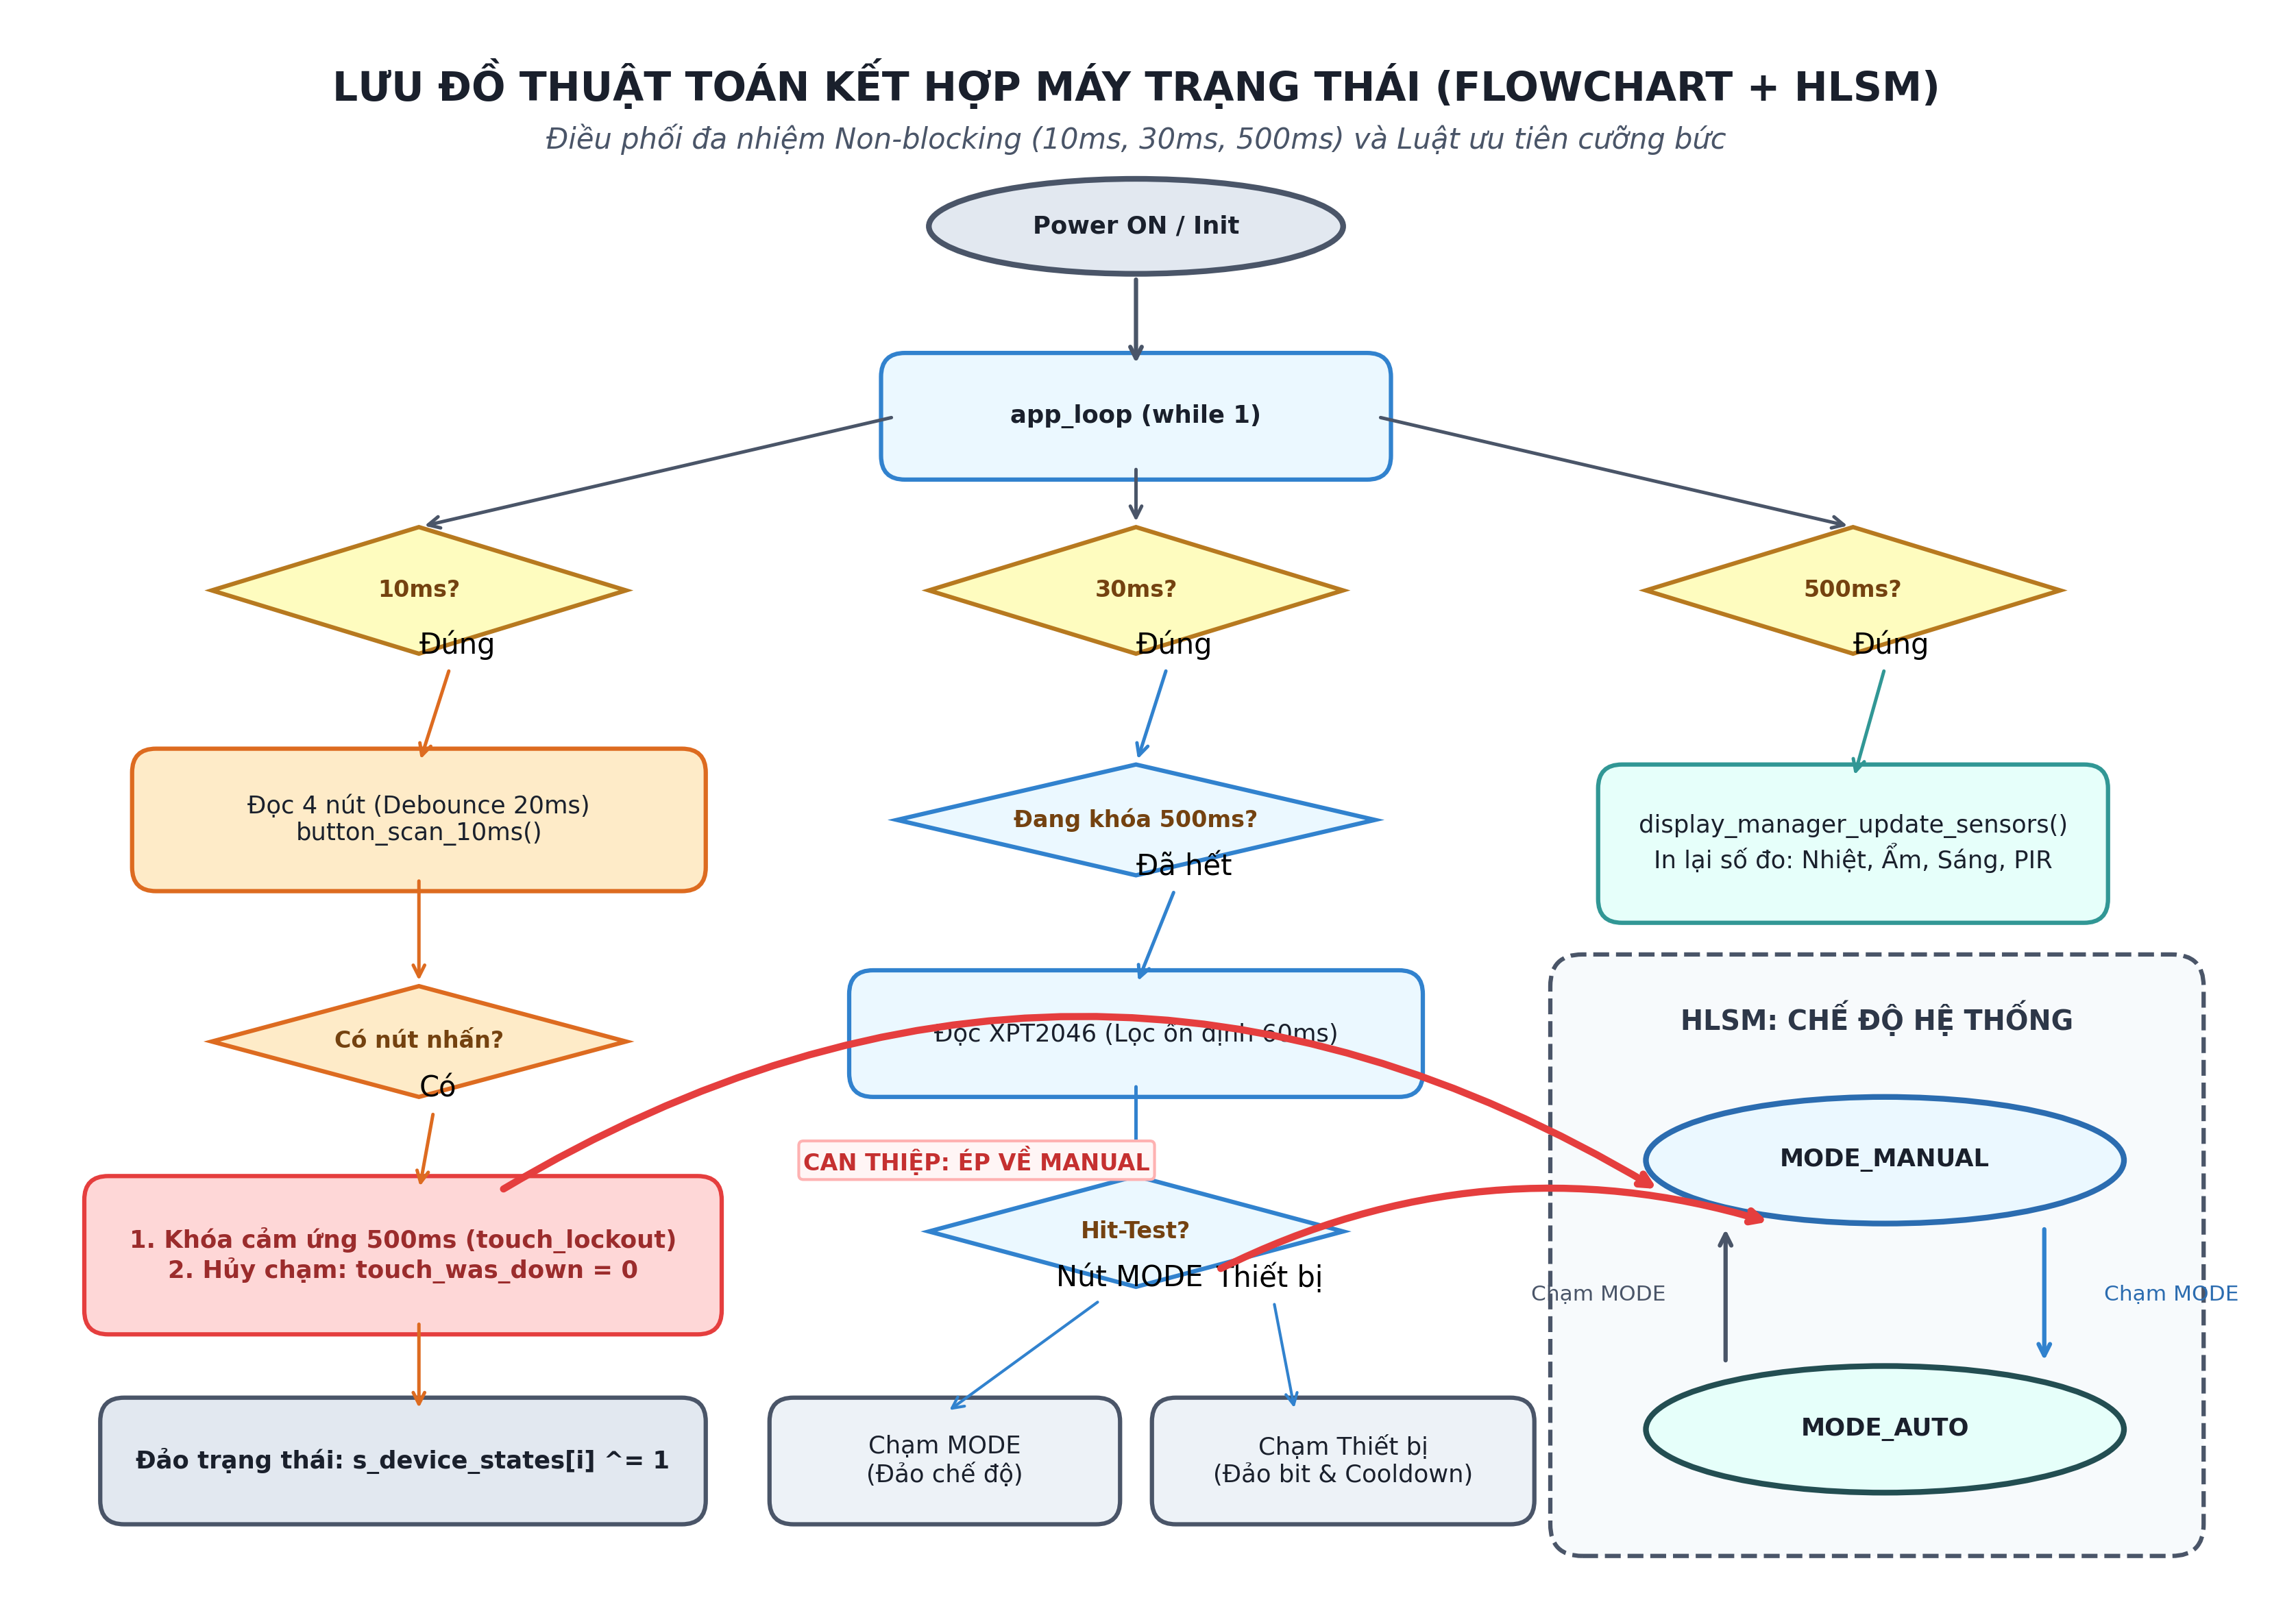
\includegraphics[width=0.98\textwidth]{figures/system_flowchart_hlsm.png}
    \caption{Lưu đồ thuật toán Scheduler kết hợp Máy trạng thái HLSM và cơ chế khóa ưu tiên}
    \label{fig:flowchart_hlsm}
\end{figure}

\section{Nguyên lý Vận hành Trọng tâm}
\begin{enumerate}
    \item \textbf{Định thời Non-blocking (Scheduler 10ms / 30ms / 500ms):}
    \begin{itemize}
        \item \textbf{Slot 10ms (Nút bấm):} Lọc rung 20ms $\to$ Đảo bit thiết bị $\to$ Ép về \texttt{MANUAL} $\to$ \textbf{Khóa cảm ứng 500ms} (\texttt{touch\_lockout\_until}). Nút bấm có độ ưu tiên cao nhất.
        \item \textbf{Slot 30ms (Cảm ứng):} Kiểm tra khóa 500ms $\to$ Lọc rung 2 mẫu liên tiếp (60ms) $\to$ Hồi chiêu 350ms $\to$ Nhận diện vùng chạm (Hit-test).
        \item \textbf{Slot 500ms (Hiển thị):} In lại chuỗi số đo cảm biến (Nhiệt, Ẩm, Sáng, PIR) mà không vẽ lại toàn màn hình (Differential Redraw chống nháy).
    \end{itemize}

    \item \textbf{Máy trạng thái HLSM \& Luật Ưu tiên Cưỡng bức (Preemption):}
    \begin{itemize}
        \item \texttt{MODE\_MANUAL}: Con người điều khiển qua nút bấm hoặc cảm ứng; cảm biến chỉ hiển thị.
        \item \texttt{MODE\_AUTO}: Tự động điều khiển Quạt ($T \ge 28^\circ\text{C}$), Hút ẩm ($H \ge 70\%$), Đèn 1 \& 2 (PIR + LDR).
        \item \textbf{Đường can thiệp màu đỏ (Cưỡng bức):} Bất kỳ thao tác nút vật lý hoặc chạm vào ô thiết bị nào khi đang ở \texttt{AUTO} sẽ lập tức ép hệ thống quay về \texttt{MANUAL} để đảm bảo an toàn.
    \end{itemize}
\end{enumerate}

\section{Bảng Ngưỡng Điều khiển Tự động (Auto Mode)}
\begin{table}[H]
\centering
\small
\begin{tabular}{@{}lllll@{}}
\toprule
\textbf{Thiết bị} & \textbf{Cảm biến} & \textbf{Ngưỡng BẬT} & \textbf{Ngưỡng TẮT} & \textbf{Độ trễ (Hysteresis)} \\ \midrule
\textbf{Quạt (PB5)} & DHT22 ($T$) & $\ge 28.0^\circ\text{C}$ & $\le 26.5^\circ\text{C}$ & $1.5^\circ\text{C}$ trễ chống rung relay \\
\textbf{Hút ẩm (PB8)} & DHT22 ($H$) & $\ge 70.0\%$ & $\le 60.0\%$ & $10.0\%$ trễ quán tính ẩm \\
\textbf{Đèn 1 (PB6)} & PIR + LDR & PIR=1 \& ADC $\ge 2000$ & Hết 5 phút PIR hoặc ADC $\le 1700$ & 300 count hysteresis \\
\textbf{Đèn 2 (PB7)} & PIR + LDR & PIR=1 \& ADC $\ge 3000$ & Hết 5 phút PIR hoặc ADC $\le 2700$ & 300 count hysteresis \\ \bottomrule
\end{tabular}
\end{table}

\end{document}
